\documentclass[12pt]{article}
\usepackage{amsthm,amssymb,amsfonts,amsmath,amstext,systeme}
\usepackage{graphicx,float}
\usepackage{tabularx}

\marginparwidth 0pt
\oddsidemargin -1.2 truecm
\evensidemargin  0pt 
\marginparsep 0pt
\topmargin -2.2truecm
\linespread{1}
\textheight 25.8 truecm
\textwidth 18.5 truecm
\newenvironment{remark}{\noindent{\bf Remark }}{\vspace{0mm}}
\newenvironment{remarks}{\noindent{\bf Remarks }}{\vspace{0mm}}
\newenvironment{question}{\noindent{\bf Question }}{\vspace{0mm}}
\newenvironment{questions}{\noindent{\bf Questions }}{\vspace{0mm}}
\newenvironment{note}{\noindent{\bf Note }}{\vspace{0mm}}
\newenvironment{summary}{\noindent{\bf Summary }}{\vspace{0mm}}
\newenvironment{back}{\noindent{\bf Background}}{\vspace{0mm}}
\newenvironment{conclude}{\noindent{\bf Conclusion}}{\vspace{0mm}}
\newenvironment{concludes}{\noindent{\bf Conclusions}}{\vspace{0mm}}
\newenvironment{dill}{\noindent{\bf Description of Dill's model}}{\vspace{0mm}}
\newenvironment{maths}{\noindent{\bf Mathematics needed}}{\vspace{0mm}}
\newenvironment{inst}{\noindent{\bf Instructions}}{\vspace{0mm}}
\newenvironment{notes}{\noindent{\bf Notes }}{\vspace{0mm}}
\newenvironment{theorem}{\noindent{\bf Theorem }}{\vspace{0mm}}
\newenvironment{example}{\noindent{\bf Example }}{\vspace{0mm}}
\newenvironment{examples}{\noindent{\bf Examples }}{\vspace{0mm}}
\newenvironment{topics}{\noindent{\bf Topics}}{\vspace{0mm}}
\newenvironment{outcomes}{\noindent{\bf Expected Learning Outcomes}}{\vspace{0mm}}
\newenvironment{lemma}{\noindent{\bf Lemma }}{\vspace{0mm}}
\newenvironment{solution}{\noindent{\it Solution}}{\vspace{2mm}}
\newcommand{\ds}{\displaystyle}
\newcommand{\un}{\underline}
\newcommand{\bs}{\boldsymbol}

\begin{document}

\baselineskip 18 pt
\begin{center}
	{\large \bf HKDSE MATH M2 2012}\\
	\vspace{2 mm}

\end{center}
\vspace{0.05cm}

\begin{enumerate}
	\item \textbf{HKDSE Math M2 2012 Q1}\\
	Let $f(x) = e^{2x}$. Find $f'(0)$ from first principles. \\(3 marks)


	\item \textbf{HKDSE Math M2 2012 Q2}\\
	It is given that 
	$$(1+ax)^n = 1 + 6x + 16x^2 +\text{terms involving higher powers of }x,$$
	where $n$ is a positive integer and $a$ is a constant. Find the values of $a$ and $n$.\\(5 marks)


	\item \textbf{HKDSE Math M2 2012 Q3}\\
	Prove, by mathematical induction, that for all positive integers $n$,\\
		$\displaystyle 1 \times 2 + 2 \times 5 + 3 \times 8 + \cdots + n(3n-1) = n^2(n+1)$. \\(5 marks)
		

	\item \textbf{HKDSE Math M2 2012 Q4}
	\begin{enumerate}
		\item [(a)]Find $\displaystyle\int \frac{x+1}{x}\,dx$
		\item [(b)]Using the substitution $u = x^2-1$, find $\displaystyle\int\frac{x^3}{x^2 - 1}\,dx$.
	\end{enumerate}
	(5 marks)

	\item \textbf{HKDSE Math M2 2012 Q5}\\
	Find the minimum point(s) and asymptote(s) of the graph of $\displaystyle y = \frac{x^2+x+1}{x+1}$. \\(6 marks)

	\item \textbf{HKDSE Math M2 2012 Q6}\\
	A frustum of height $H$ is made by cutting off a right circular cone of base radius $r$ from a right circular cone of base radius $R$ (See Figure 1). It is given that the volume of the frustum is $\displaystyle\frac{\pi}{3}H(r^2 + rR + R^2)$. \\
	An empty glass is in the form of an inverted frustum described above with height 10 cm, the radii of the rim and the base 4 cm and 3 cm respectively. Water is being poured into the glass. Let $h$ cm $(0 \leq h \leq 10)$ be the depth of the water inside the glass at time $t$ s (see Figure 2).
	\begin{figure}[H]
		\centering
		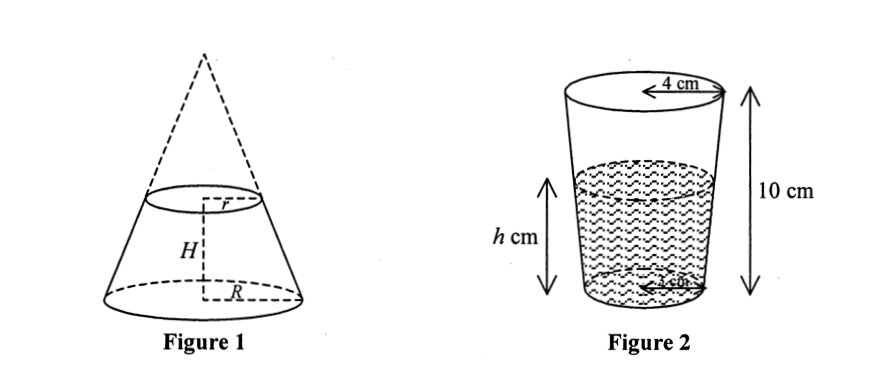
\includegraphics[width = .5\linewidth]{2012Figure1n2}
	\end{figure}
	\begin{enumerate}
		\item [(a)]Show that the volume $V$ cm$^{3}$ of water inside the glass at time $t$ s is given by \\
		$V = \displaystyle\frac{\pi}{300}(h^3+90h^2+2700h)$. 
		\item [(b)]If the volume of water in the glass is increasing at the rate $7\pi$ cm$^3$ s$^{-1}$, find the rate of increase of depth of water at the instant when $h = 5$.
	\end{enumerate}
	(6 marks)

	\item \textbf{HKDSE Math M2 2012 Q7}\\
	Figure 3 shows a parallelepiped $OADBECFG$. Let $\overrightarrow{OA} = 6\textbf{i} +2\textbf{j} -\textbf{k}$, $\overrightarrow{OB} = 2\textbf{i} +\textbf{j} $ and $\overrightarrow{OC} = 5\textbf{i} -\textbf{j} +2\textbf{k}$.
	\begin{figure}[H]
		\centering
		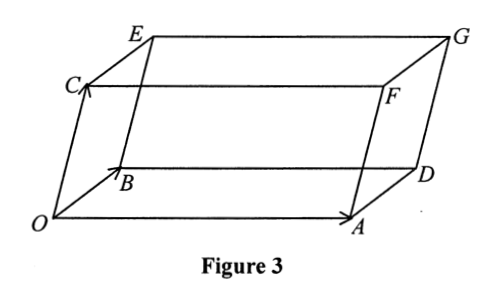
\includegraphics[width = .5\linewidth]{2012Figure3}
	\end{figure}
	\begin{enumerate}
		\item [(a)]Find the area of the parallelogram $OADB$. 
		\item [(b)]Find the distance between point $C$ and the plane $OADB$.
	\end{enumerate}
	(5 marks)

	\item \textbf{HKDSE Math M2 2012 Q8}
	\begin{enumerate}
		\item [(a)]Solve the following system of linear equations:
		$$\left\{\begin{matrix}
			x & + & y & + & z & = & 0\\
			2x & - & y & + & 5z & = & 6\\
		\end{matrix}\right.$$
		\item [(b)]Using (a), or otherwise, solve the following system of linear equations: 
		$$\left\{\begin{matrix}
			x & + & y & + & z & = & 0\\
			2x & - & y & + & 5z & = & 6\\
			x & - & y & + & \lambda z & = & 4\\
		\end{matrix}\right.\text{ , where }\lambda\text{ is a constant.}$$ 
	\end{enumerate}
	(5 marks)

	\item \textbf{HKDSE Math M2 2012 Q9}
	\begin{enumerate}
		\item [(a)]Using integration by parts, find $\int x\sin{x}\,dx$. 
		\item [(b)]Figure 4 shows the shaded region bounded by the curve $y = \sqrt{x\sin{x}}$ for $0 \leq x \leq \pi$ and the $x$-axis. Find the volume of the solid generated by revolving the region about the $x$-axis.
	\begin{figure}[H]
		\centering
		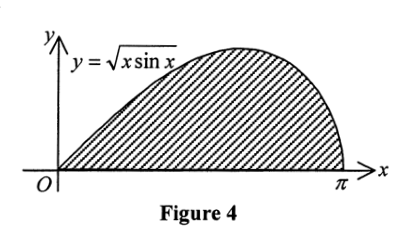
\includegraphics[width = .5\linewidth]{2012Figure4}
	\end{figure}
	\end{enumerate}
	(4 marks)


	\item \textbf{HKDSE Math M2 2012 Q10}\\
	In Figure 5, $OAB$ is an isosceles triangle with $OA = OB$, $AB = 1$, $AY = y$, $\angle AOY = \theta$ and $\angle BOY = 3\theta$. 
	\begin{figure}[H]
		\centering
		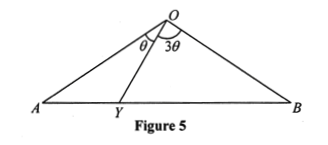
\includegraphics[width = .5\linewidth]{2012Figure5}
	\end{figure}
	\begin{enumerate}
		\item [(a)]Show that $y = \displaystyle\frac{1}{4}\sec^2{\theta}$.
		\item [(b)]Find the range of values of $y$. [Hint: you may use the identity $\sin{3\theta} = 3\sin{\theta} - 4\sin^3{\theta}$.]
	\end{enumerate}
	(6 marks)

	\item \textbf{HKDSE Math M2 2012 Q11}
	\begin{enumerate}
		\item [(a)]Solve the equation \\$\begin{vmatrix}
			1-x & 4  \\ 
			2 & 3-x  \notag
		\end{vmatrix} = 0 $ --------------(*). \\(2 marks)
		\item [(b)]Let $x_1 ,\, x_2  $ $(x_1<x_2)$ be the roots of (*). Let $P = \begin{pmatrix}
			a&c\\b&1\\
		\end{pmatrix}$. It is given that \\
		$\begin{pmatrix}1&4\\2&3\\\end{pmatrix}\begin{pmatrix}a\\b\\\end{pmatrix} = x_1 \begin{pmatrix}a\\b\\\end{pmatrix}$, $\begin{pmatrix}1&4\\2&3\\\end{pmatrix}\begin{pmatrix}c\\1\\\end{pmatrix} = x_2 \begin{pmatrix}c\\1\\\end{pmatrix}$ and $|P| =1$,\\
		where $a$, $b$ and $c$ are constants.
		\begin{enumerate}
			\item [(i)]Find $P$.
			\item [(ii)]Evaluate $P^{-1}\begin{pmatrix}1&4\\2&3\\\end{pmatrix}P$.
			\item [(iii)]Using (b)(ii), evaluate $\begin{pmatrix}1&4\\2&3\\\end{pmatrix}^{12}$.
		\end{enumerate}
		(11 marks)
	\end{enumerate}


	\item \textbf{HKDSE Math M2 2012 Q12}\\
	Figure 6 shows an acute angled scalene triangle $ABC$, where $D$ is the mid-point of $AB$, $G$ is the centroid and $O$ is the circumcentre. Let $\overrightarrow{OA} = \textbf{a}$, $\overrightarrow{OB} = \textbf{b}$ and $\overrightarrow{OC} = \textbf{c}$.
	\begin{figure}[H]
		\centering
		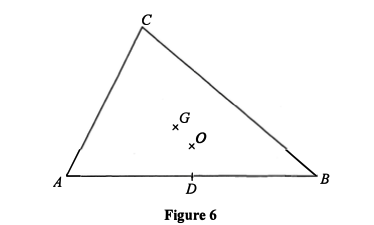
\includegraphics[width = .5\linewidth]{2012Figure6}
	\end{figure}
	\begin{enumerate}
		\item [(a)]Express $\overrightarrow{AG}$ in terms of $\textbf{a}$, $\textbf{b}$ and $\textbf{c}$.\\(3 marks)
		\item [(b)]It is given that $E$ is a point on $AB$ such that $CE$ is an altitude. Extend $OG$ to meet $CE$ at $F$. 
		\begin{enumerate}
			\item [(i)]Prove that $\triangle DOG \sim \triangle CFG$. \\Hence find $FG:GO$. 
			\item [(ii)]Show that $\overrightarrow{AF} = \textbf{b} + \textbf{c}$. \\Hence prove that $F$ is the orthocentre of $\triangle ABC$.
		\end{enumerate}
		(9 marks)
	\end{enumerate}

	\item \textbf{HKDSE Math M2 2012 Q13}
	\begin{enumerate}
		\item [(a)]
		\begin{enumerate}
			\item [(i)]Suppose $\tan{u} = \displaystyle\frac{-1 + \cos{\displaystyle\frac{2\pi}{5}}}{\sin{\displaystyle\frac{2\pi}{5}}}$, where $\displaystyle\frac{-\pi}{2} < u < \frac{\pi}{2}$. \\
			Show that $u = \displaystyle\frac{-\pi}{5}$. 
			\item [(ii)]Suppose $\tan{v} = \displaystyle\frac{1+\cos{\displaystyle\frac{2\pi}{5}}}{\sin{\displaystyle\frac{2\pi}{5}}}$. \\
			Find $v$, where $\displaystyle\frac{-\pi}{2} < v < \frac{\pi}{2}$.
		\end{enumerate}
		(4 marks)
		\item[(b)]
		\begin{enumerate}
			\item[(i)]Express $x^2 + 2x\cos{\displaystyle\frac{2\pi}{5}} + 1$ in the form $(x+a)^2 + b^2$, where $a$ and $b$ are constants. 
			\item[(ii)]Evaluate $\displaystyle\int_{-1}^{1}\frac{\sin{\displaystyle\frac{2\pi}{5}}}{x^2 + 2x\cos{\displaystyle\frac{2\pi}{5}}+1}\, dx$.
		\end{enumerate}
		(6 marks)
		\item[(c)]Evaluate $\displaystyle\int_{-1}^{1}\frac{\sin{\displaystyle\frac{7\pi}{5}}}{x^2 + 2x\cos{\displaystyle\frac{7\pi}{5}}+1} \,dx$. \\(3marks)
	\end{enumerate}


	\item \textbf{HKDSE Math M2 2012 Q14}\\
	Consider the curve $\Gamma : y = kx^p$, where $k>0$, $p > 0$. In Figure 7, the tangent to $\Gamma$ at $A(a, ka^{p})$ cuts the $x$-axis at $B(-a, 0)$, where $a>0$.
	\begin{figure}[H]
		\centering
		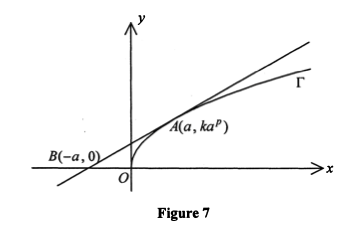
\includegraphics[width = .5\linewidth]{2012Figure7}
	\end{figure}
	\begin{enumerate}
		\item [(a)]Show that $\displaystyle p = \frac{1}{2}$. \\(3 marks)
		\item [(b)]Suppose that $a = 1$. As shown in Figure 8, the circle $C$, with radius 2 and centre on the $y$-axis, touches $\Gamma$ at point $A$.
		\begin{figure}[H]
			\centering
			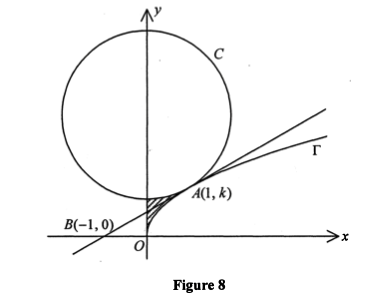
\includegraphics[width = .5\linewidth]{2012Figure8}
		\end{figure}
		\begin{enumerate}
			\item [(i)]Show that $\displaystyle k = \frac{2\sqrt{3}}{3}$. 
			\item [(ii)]Find the area of the shaded region bounded by $\Gamma$, $C$ and the $y$-axis.
		\end{enumerate}
		(9 marks)
	\end{enumerate}
\end{enumerate}
\end{document}